\documentclass[zihao = -4,linespread = 1.38889, heading = true,no-math]{ctexbook} %定义文档类型,请勿修改
% ---------------------------
\usepackage{packages/gscaepthesis}

% 编译方式 : XeLaTeX ——> Biber ——> XeLaTeX *2 
% 使用bibtex而不用Biber的话可能会导致文献格式错误.
% 文件夹中内嵌了所需的字体,如果电脑系统安装了这些字体,可以删掉;已经按照院里要求的格式把字体以及字号都设置好,理论上不需要额外修改字体了

% 随机文本生成器-用于测试文本效果 - 实际写作中请去掉
\usepackage{lipsum}
\usepackage{zhlipsum}



% ---------------------------------------------------------------------------
% 论文的基本信息
\classificationnumber{ }%分类号
\confidentialitylevel{公开}%秘级,不加这一行默认为公开
\thesisudc{ }%在此填写udc
\thesisnum{ }%在此填写编号

\cntitle{中国工程物理研究院研究生院学位论文模板}%中文标题
\entitle{GASCEP Thesis \LaTeX Template}%英文标题
\cnauthor{翟若迅}%中文作者
\enauthor{Ruo-Xun Zhai}%英文作者


\supervisornamecn{xxx}{教授/研究员} %中文导师;第一个参数为姓名,第二个参数为职称
\supervisornameen{xxx}{Prof.} %英文导师;第一个参数为姓名,第二个参数为职称

%----------------------------
% 申请学位的等级,若无代码规定,则该行默认为理学博士学位,下列四行中请只保留一行
\doctorofscience %理学博士
% \doctorofengineering % 工学博士
% \masterofscience % 理学硕士
% \masterofengineering % 工学硕士
%----------------------------

\fieldofstudycn{理论物理} %中文专业名称 —— 需与学生学籍信息保持一致
\fieldofstudyen{Theoretical Physics} % 二级学科的英文名称(比如Materials Science and Engineering)

% ---------------------------
% 日期设置
% 日期请严格按照例子中的格式填写,即 yyyy/mm/dd ,模板会自动转化为符合要求的格式,不要自己填别的,填别的会造成编译失败

\dateofsubmmit{2024/04/15} %论文提交日期
\dateofdefense{2024/05/15} %论文答辩日期
\thesisdate{2024/05/16}%论文日期:答辩日期和分委员会会议之间
% ---------------------------

%答辩委员会主席
\chairman{XXX}
%评阅人
\reviewer{YYY}

% ---------------------------------------------------------------------------

%以下为正文部分
\begin{document}

\makecover % 打印封面

% --------------------------------------------------------------------------
%定义摘要和关键词,请务必保证定义关键词的命令在摘要之前出现
\keywordscn{关键词1,关键词2,关键词3} %中文关键词
\keywordsen{Keyword 1, Keyword 2, Keyword 3} %英文关键词

\begin{cnabstract}
  \zhlipsum[1-2]% 将此行替换为中文摘要
\end{cnabstract}


\begin{enabstract}
  \lipsum[1-3]% 将此行替换为英文摘要
\end{enabstract}


\tableofcontents
\cleardoublepage

\pagenumbering{arabic}
\setcounter{page}{1}
\chapter{引言}
\zhlipsum[1]

\chapter{一级标题}
\zhlipsum[1]
\section{二级标题}
\zhlipsum[1-3]
\subsection{三级标题}
\zhlipsum[1]
\subsection{三级标题}
\subsubsection{四级标题}
\zhlipsum[1-2]
\begin{figure}
  \centering
  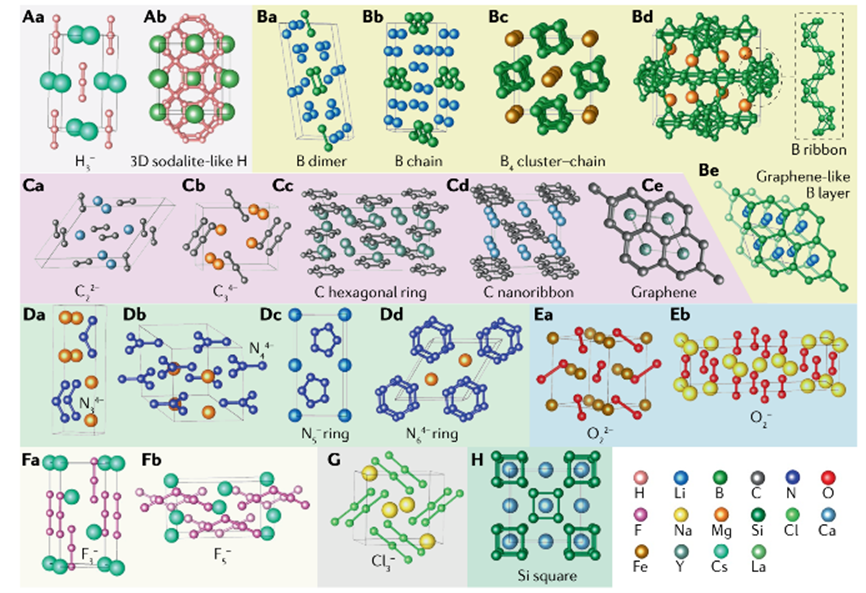
\includegraphics[width = 14cm]{figs/ThisFigure.png}
  \caption{这是一个简单的图片示例}
\end{figure}
\zhlipsum[3-5]


\begin{equation}
  PV = nRT,
\end{equation}
\begin{equation}
  E = mc^2.
\end{equation}


\chapter{一级标题}
\zhlipsum[1]
\begin{equation}
  E = mc^2.
\end{equation}


\section{二级标题}
\zhlipsum[1-3]
\subsection{三级标题}
\zhlipsum[1-3]
\begin{table}
  \centering
  \caption{这是一个简单的表格示例}
  \vspace{0.5em}
  \begin{tabular}{ccc}
    \hline
    \hline
    列1 & 列2 & 列3 \\
    \hline
    数据1 & 数据2 & 数据3 \\
    数据4 & 数据5 & 数据6 \\
    \hline
  \end{tabular}
\end{table}

\chapter{一级标题}
\zhlipsum[1]
\section{二级标题}
\zhlipsum[1-3]
\subsection{三级标题}
\zhlipsum[1-3]

参考文献测试:引用书籍\cite{Guiner1982},引用期刊\cite{Canvendish1985},引用学位论文\cite{Cao1993},引用论文集\cite{Jin1993}. 测试脚注\cite{footnote01}.
请大家在reference.bib中参照格式查看并编辑参考文献!


% 打印参考文献
\printbibgscaep

\begin{acknowledgements}
  \zhlipsum[1] %中间写致谢
\end{acknowledgements}

\gscaepappendix % 开始附录
%附录中的一级标题请使用section,而不要再使用chapter

\section{论文相关的补充图、表及公式推导}
\subsection{二级标题}
\zhlipsum[1]
\subsubsection{三级标题}
\zhlipsum[1]
\subsection{二级标题}
\zhlipsum[1-2]
\subsection{二级标题}
\zhlipsum[1-2]

\section{在校期间发表学术论文、参加学术活动及各种获奖情况}
\subsection{第一篇}
\zhlipsum[1]

\subsection{第二篇}
\zhlipsum[1]

\end{document}